\documentclass{article}%
\usepackage[T1]{fontenc}%
\usepackage[utf8]{inputenc}%
\usepackage{lmodern}%
\usepackage{textcomp}%
\usepackage{lastpage}%
\usepackage{geometry}%
\geometry{margin=0.5in}%
\usepackage{graphicx}%
%
\title{Report on Weather Australia dataset}%
\author{Auto2Class}%
%
\begin{document}%
\normalsize%
\maketitle%
\newpage%
\tableofcontents%
\newpage%
\section{Exploratory Data Analysis}%
\label{sec:ExploratoryDataAnalysis}%
\subsection{Non{-}Null Count, Dtype of features}%
\label{subsec:Non{-}NullCount,Dtypeoffeatures}%


\begin{table}[h!]%
\caption{Dataset Columns Information}%
\vspace{0.2cm}%
\centering%
\begin{tabular}{|c||c||c||c|}%
\hline%
Index&Column&Non{-}Null Count&Dtype\\%
\hline%
0&Date&145460&object\\%
1&Location&145460&object\\%
2&MinTemp&143975&float64\\%
3&MaxTemp&144199&float64\\%
4&Rainfall&142199&float64\\%
5&Evaporation&82670&float64\\%
6&Sunshine&75625&float64\\%
7&WindGustDir&135134&object\\%
8&WindGustSpeed&135197&float64\\%
9&WindDir9am&134894&object\\%
10&WindDir3pm&141232&object\\%
11&WindSpeed9am&143693&float64\\%
12&WindSpeed3pm&142398&float64\\%
13&Humidity9am&142806&float64\\%
14&Humidity3pm&140953&float64\\%
15&Pressure9am&130395&float64\\%
16&Pressure3pm&130432&float64\\%
17&Cloud9am&89572&float64\\%
18&Cloud3pm&86102&float64\\%
19&Temp9am&143693&float64\\%
20&Temp3pm&141851&float64\\%
21&RainToday&142199&object\\%
22&RainTomorrow&142193&object\\%
\hline%
\end{tabular}%
\end{table}

%
\subsection{Descriptive Statistics}%
\label{subsec:DescriptiveStatistics}%


\begin{table}[h!]%
\caption{Dataset Descriptive Statistics}%
\vspace{0.2cm}%
\centering%
\begin{tabular}{|c||c||c||c||c||c||c||c||c||c|}%
\hline%
Index&Column Name/Statistic&count&mean&std&min&25\%&50\%&75\%&max\\%
\hline%
0&MinTemp&143975.0&12.19&6.4&{-}8.5&7.6&12.0&16.9&33.9\\%
1&MaxTemp&144199.0&23.22&7.12&{-}4.8&17.9&22.6&28.2&48.1\\%
2&Rainfall&142199.0&2.36&8.48&0.0&0.0&0.0&0.8&371.0\\%
3&Evaporation&82670.0&5.47&4.19&0.0&2.6&4.8&7.4&145.0\\%
4&Sunshine&75625.0&7.61&3.79&0.0&4.8&8.4&10.6&14.5\\%
5&WindGustSpeed&135197.0&40.04&13.61&6.0&31.0&39.0&48.0&135.0\\%
6&WindSpeed9am&143693.0&14.04&8.92&0.0&7.0&13.0&19.0&130.0\\%
7&WindSpeed3pm&142398.0&18.66&8.81&0.0&13.0&19.0&24.0&87.0\\%
8&Humidity9am&142806.0&68.88&19.03&0.0&57.0&70.0&83.0&100.0\\%
9&Humidity3pm&140953.0&51.54&20.8&0.0&37.0&52.0&66.0&100.0\\%
10&Pressure9am&130395.0&1017.65&7.11&980.5&1012.9&1017.6&1022.4&1041.0\\%
11&Pressure3pm&130432.0&1015.26&7.04&977.1&1010.4&1015.2&1020.0&1039.6\\%
12&Cloud9am&89572.0&4.45&2.89&0.0&1.0&5.0&7.0&9.0\\%
13&Cloud3pm&86102.0&4.51&2.72&0.0&2.0&5.0&7.0&9.0\\%
14&Temp9am&143693.0&16.99&6.49&{-}7.2&12.3&16.7&21.6&40.2\\%
15&Temp3pm&141851.0&21.68&6.94&{-}5.4&16.6&21.1&26.4&46.7\\%
\hline%
\end{tabular}%
\end{table}

%
\newpage%
\subsection{Distribution of features}%
\label{subsec:Distributionoffeatures}%
\subsubsection{Histograms of Numerical columns}%
\label{ssubsec:HistogramsofNumericalcolumns}%


\begin{figure}[h!]%
\centering%
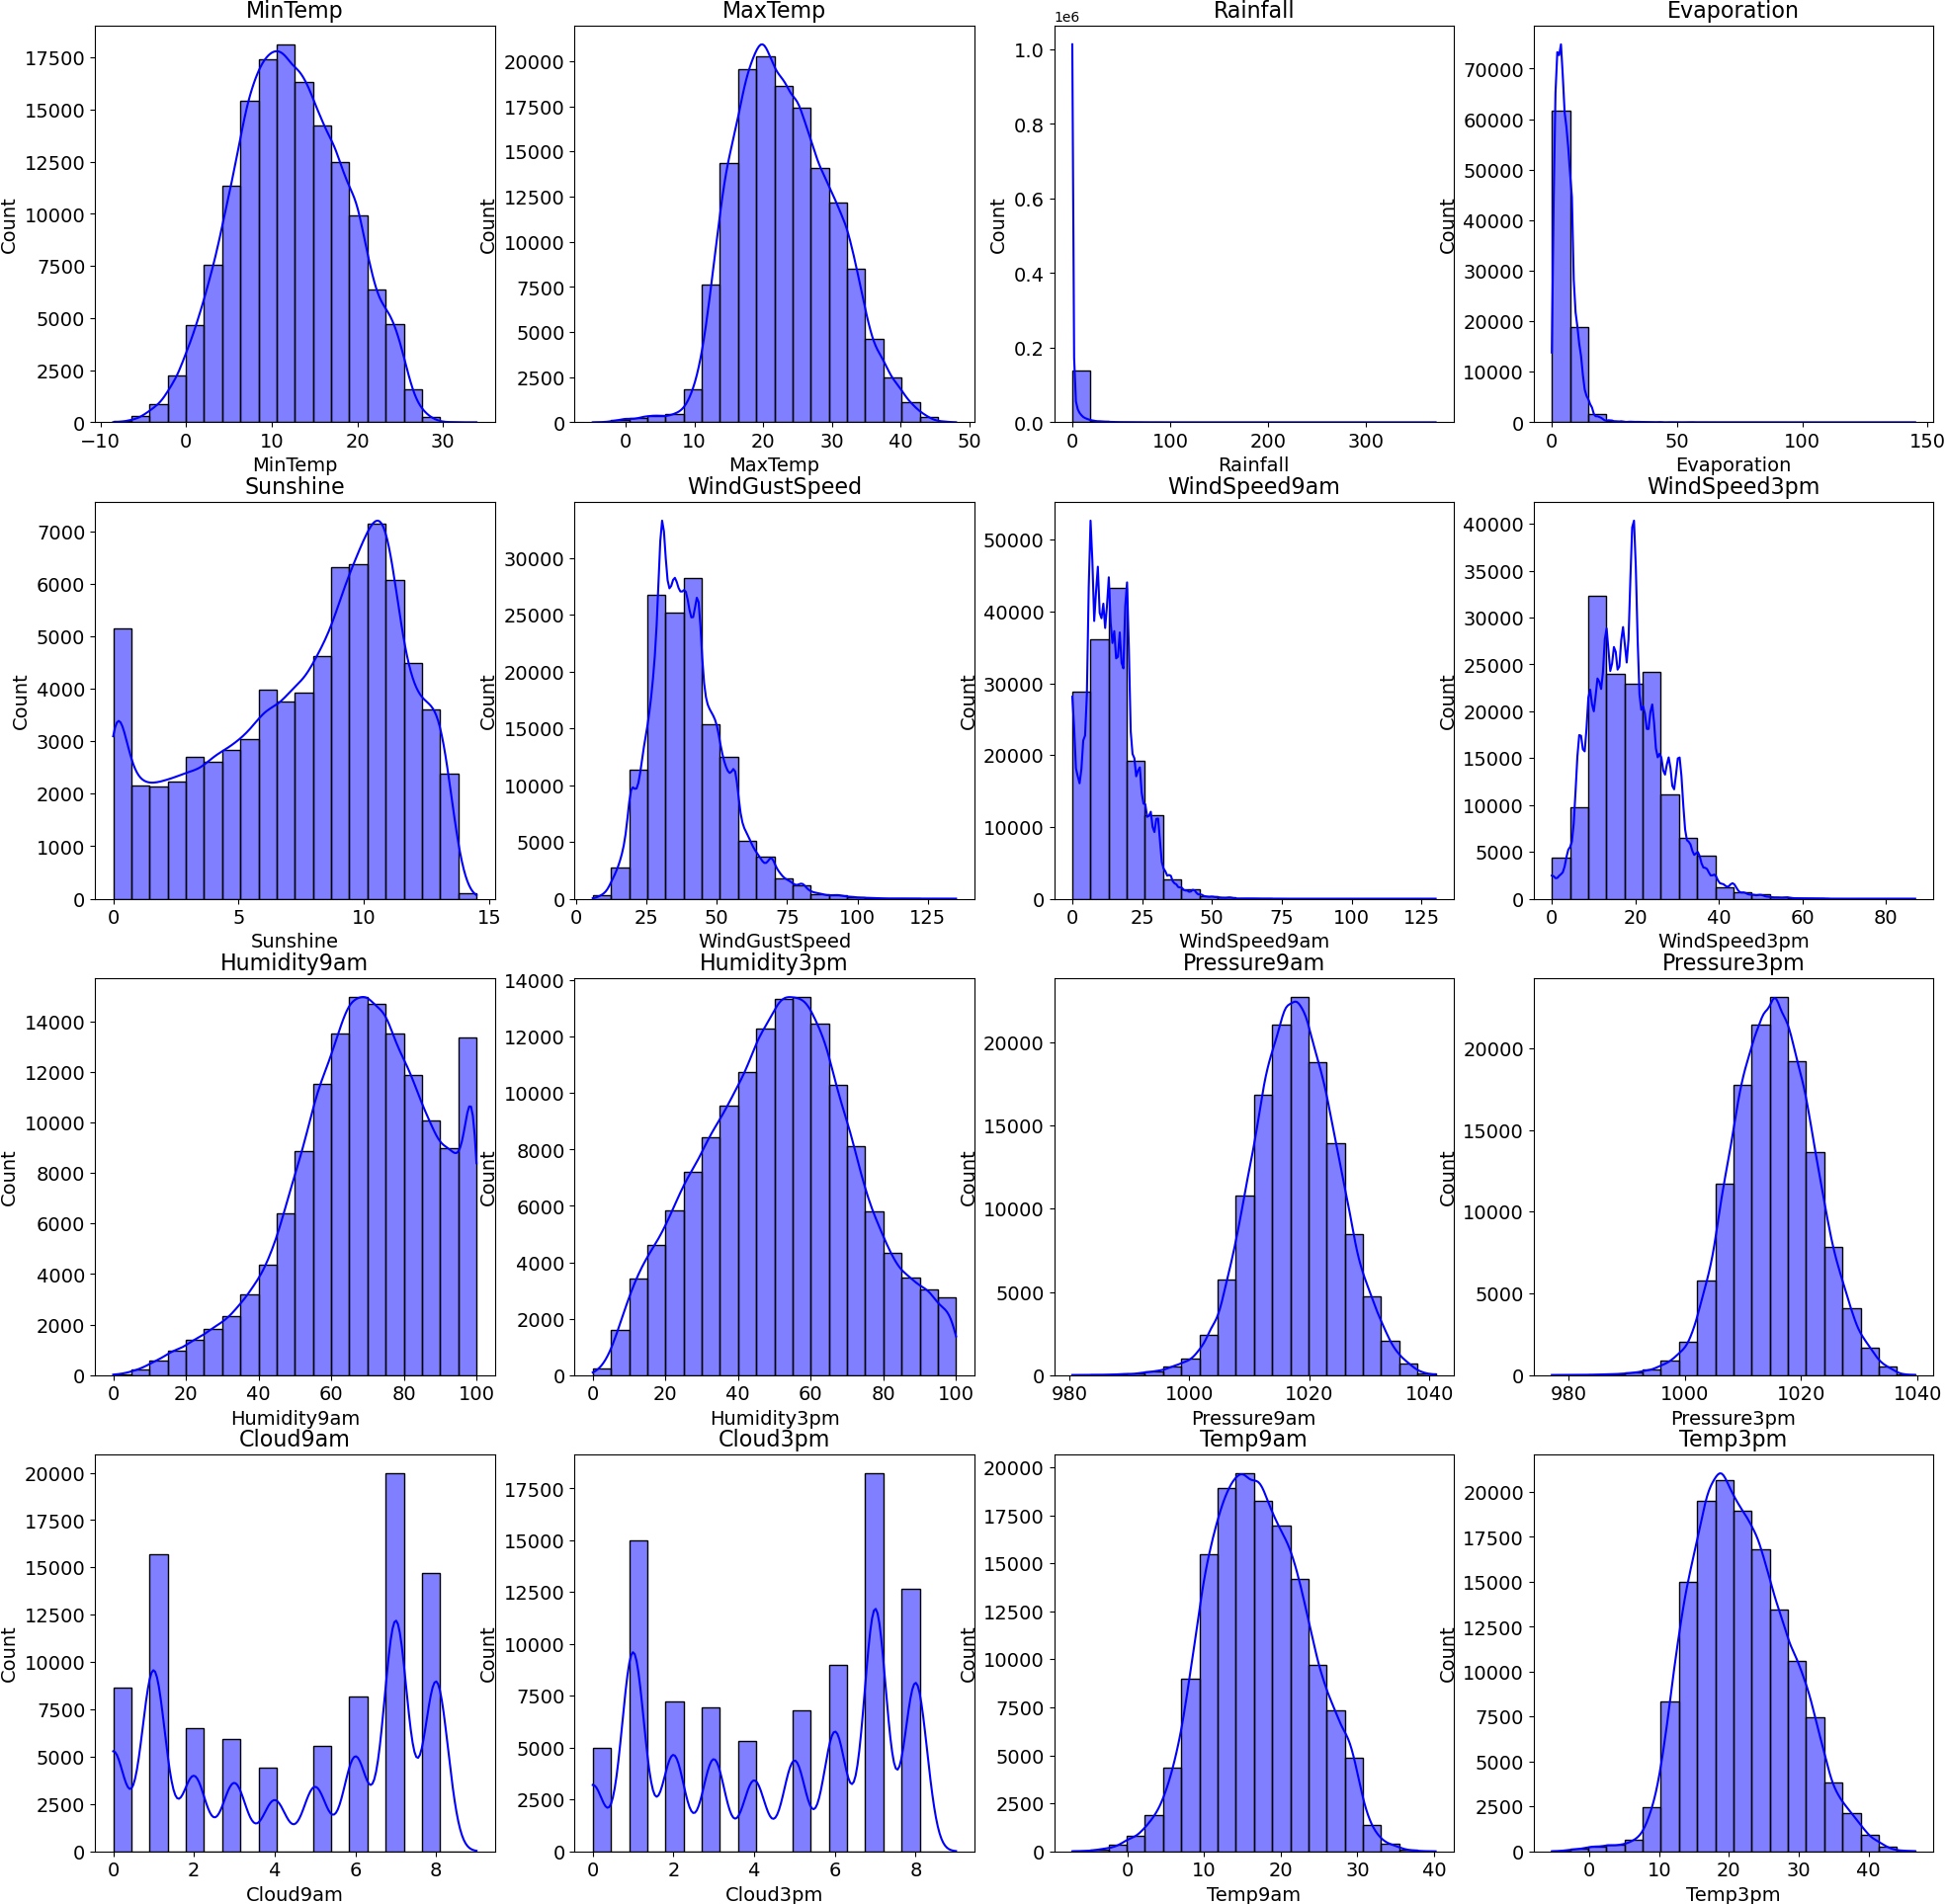
\includegraphics[width=460px]{Results/EDA/histograms.png}%
\caption{Histograms of Numerical columns}%
\end{figure}

%
\newpage%
\subsubsection{Bar Charts of Categorical columns}%
\label{ssubsec:BarChartsofCategoricalcolumns}%


\begin{figure}[h!]%
\centering%
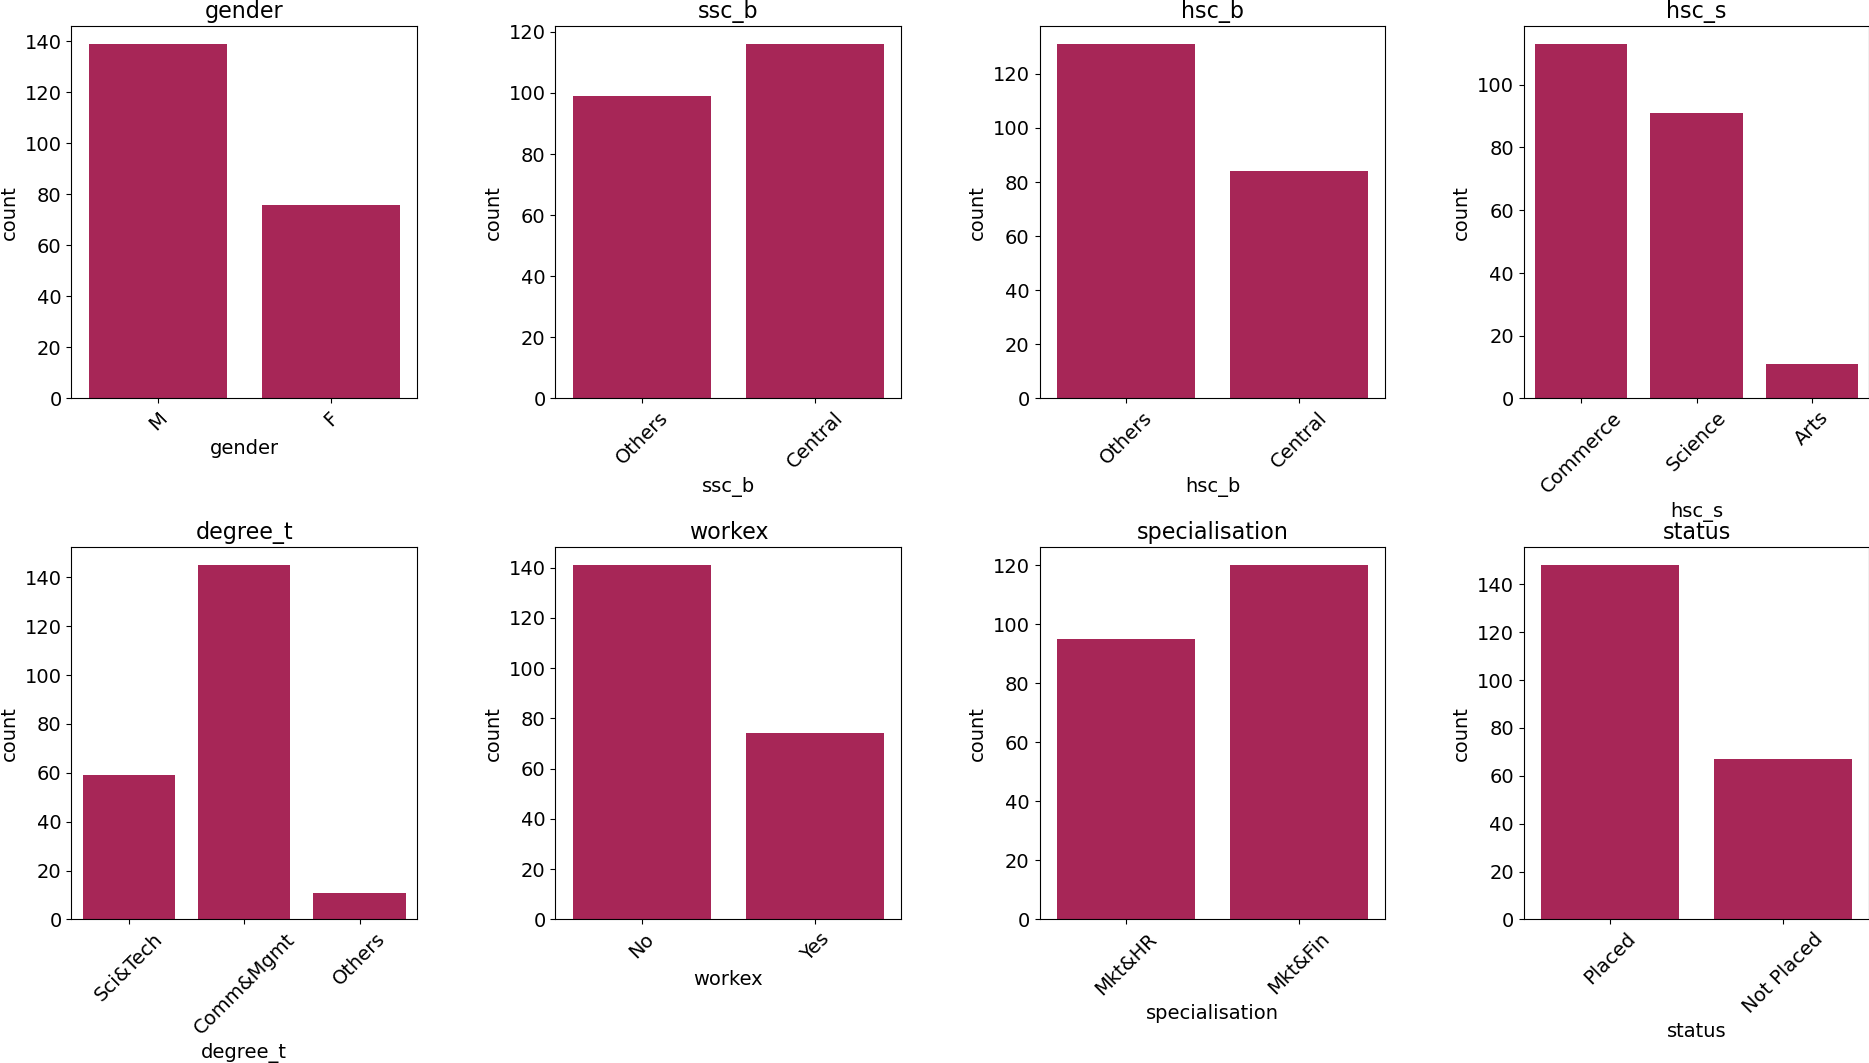
\includegraphics[width=460px]{Results/EDA/bar_charts.png}%
\caption{Bar Charts of Categorical columns}%
\end{figure}

%
\newpage%
\section{Model Optimization Results}%
\label{sec:ModelOptimizationResults}%
\subsection{Optimization Results Tables}%
\label{subsec:OptimizationResultsTables}%


\begin{table}[h!]%
\caption{Random Forest Hyperparameters and achivied metrics}%
\vspace{0.2cm}%
\centering%
\begin{tabular}{|c||c||c||c||c|}%
\hline%
Index&Metric/Hyperp.\textbackslash{} Iteration&0&1&2\\%
\hline%
0&f1&0.9314&0.7738&0.9278\\%
1&accuracy&0.9314&0.7738&0.9279\\%
2&roc\_auc&0.9837&0.8582&0.9825\\%
3&n\_estimators&100&50&50\\%
4&criterion&gini&gini&log\_loss\\%
5&max\_depth&None&20&30\\%
6&min\_samples\_split&2&2&2\\%
7&min\_samples\_leaf&1&1&1\\%
8&min\_weight\_fraction\_leaf&0.0&0.01&0.0\\%
9&max\_features&sqrt&log2&None\\%
10&bootstrap&1&1&1\\%
\hline%
\end{tabular}%
\end{table}

%


\begin{table}[h!]%
\caption{Decision Tree Hyperparameters and achivied metrics}%
\vspace{0.2cm}%
\centering%
\begin{tabular}{|c||c||c||c||c|}%
\hline%
Index&Metric/Hyperp. \textbackslash{} Iteration&0&1&2\\%
\hline%
0&f1&0.8896&0.708&0.8374\\%
1&accuracy&0.89&0.7133&0.8374\\%
2&roc\_auc&0.89&0.7135&0.8949\\%
3&criterion&gini&log\_loss&log\_loss\\%
4&splitter&best&best&best\\%
5&max\_depth&None&None&40\\%
6&min\_samples\_split&2&10&2\\%
7&min\_samples\_leaf&1&2&4\\%
8&max\_features&None&None&sqrt\\%
9&class\_weight&None&None&None\\%
10&min\_impurity\_decrease&0.0&0.1&0.0\\%
\hline%
\end{tabular}%
\end{table}

%


\begin{table}[h!]%
\caption{XGBoost Hyperparameters and achivied metrics}%
\vspace{0.2cm}%
\centering%
\begin{tabular}{|c||c||c||c||c|}%
\hline%
Index&Metric/Hyperp. \textbackslash{} Iteration&0&1&2\\%
\hline%
0&f1&0.8338&0.8263&0.7899\\%
1&accuracy&0.8339&0.8263&0.7899\\%
2&roc\_auc&0.916&0.9101&0.8753\\%
3&eval\_metric&logloss&logloss&logloss\\%
4&n\_estimators&100&50&50\\%
5&max\_depth&6&10&6\\%
6&learning\_rate&0.3&0.05&0.05\\%
7&subsample&1.0&0.7&0.5\\%
8&colsample\_bytree&1.0&0.7&0.7\\%
9&min\_child\_weight&1&1&7\\%
10&gamma&0.0&0.0&0.1\\%
11&reg\_alpha&0&1&1\\%
12&reg\_lambda&1&1&2\\%
\hline%
\end{tabular}%
\end{table}

%
\newpage%
\subsection{Boxplots of accuracy, f1, roc\_auc}%
\label{subsec:Boxplotsofaccuracy,f1,rocauc}%


\begin{figure}[h!]%
\centering%
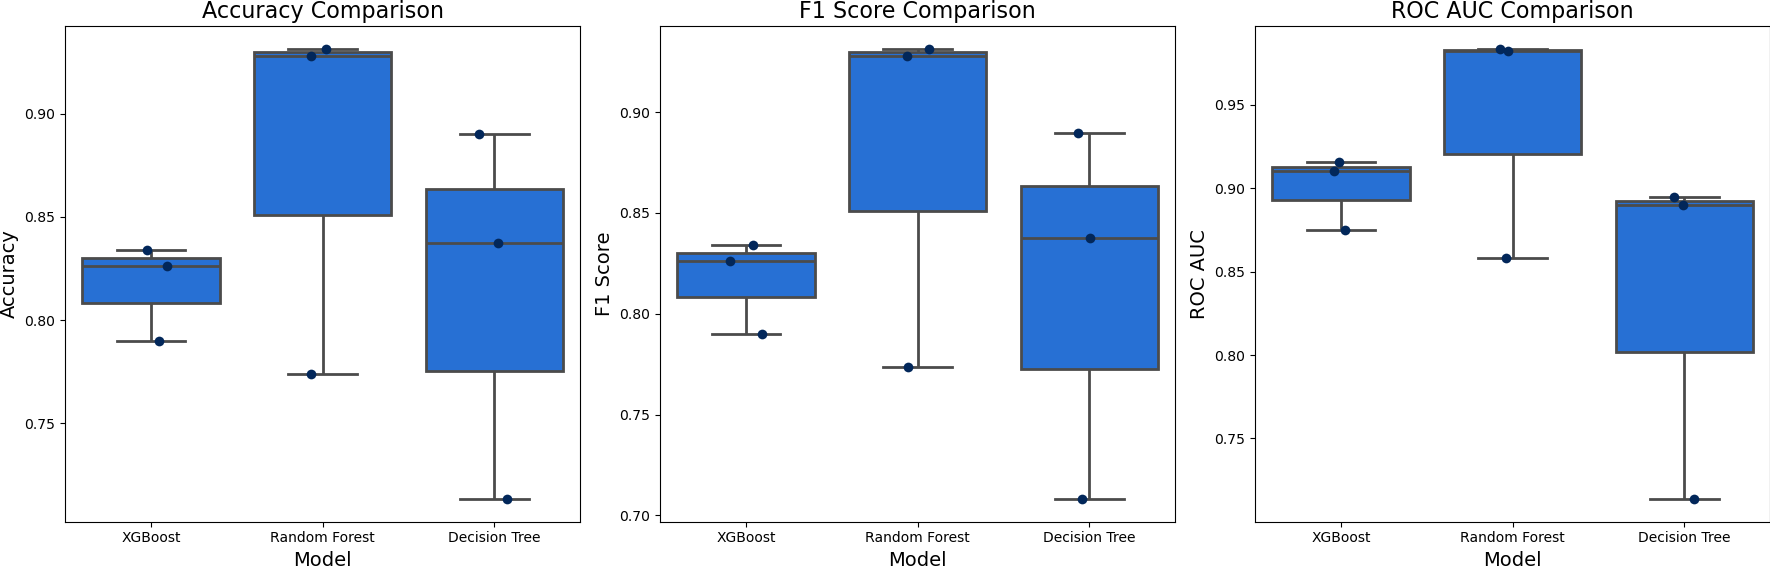
\includegraphics[width=460px]{Results/ModelOptimization/box_plots_metrics.png}%
\caption{Boxplots of accuracy, f1, roc\_auc}%
\end{figure}

%
\end{document}